\newcommand{\bbeta}{\boldsymbol\beta}
\newcommand{\trans}{^\mathsf{T}}
% \newcommand{\given}{\!\mathrel{\big|}\!}
\newcommand{\softmax}{\mathscr{S}}      % Softmax
\newcommand{\cat}{\text{Cat}}
\newcommand{\logistic}{\text{sigm}}

\lab{Logistic Regression}{Logistic Regression}
\objective{Understand the basic principles of Logistic Regression and binary classifiers. Apply this to a dataset.}

Linear regression is unsuitable for predicting probabilities, because the resulting model may take values in any fixed interval in $\mathbb{R}$, but a probability-predicting model can only take values in the interval $[0,1]$.
\emph{Logistic regression} is a form of regression that always takes its values in the interval $[0,1]$ and as such, is a popular method for predicting probabilities and for constructing \emph{classifiers}.
As in linear regression, in a classification problem we have a random variable $Y$, conditioned on an input $X \in \mathbb{R}^d$. 
However, in \emph{binary classification} problems the random variable $Y$ is binary, that is, $Y\in\{0,1\}$.   
A \emph{binary classifier} is any function $f$ taking values in $\{0,1\}$. 
For example, $\x\in \mathbb{R}^d$ could be the pixel intensities of an image, and the classifier $f$ gives $1$ if the image is a picuture of a duck and $0$ otherwise.  
The goal of a classification problem is to choose a classifier $\widehat{f}$ so that $(X,\widehat{f}(X))$ is a good approximation for $(X,Y)$.

\section*{Logistic Regression}
Logistic regression relies heavily on the \emph{logistic function}, also known as the \emph{sigmoid function}, $\text{sigm} : \mathbb{R} \rightarrow (0,1)$ given by
\begin{equation}\label{eq:logistic}
\text{sigm}(x) = \frac{1}{1 + e^{-x}}.
\end{equation}

\begin{figure}[H]
    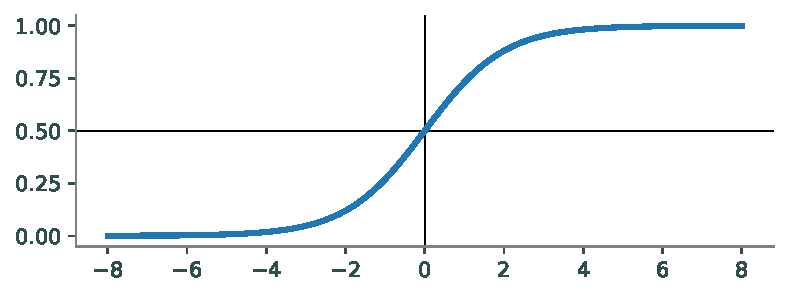
\includegraphics[width=.7\textwidth]{figures/sigmoid.pdf}
    \caption{Sigmoid Function}
\end{figure}

This function works well for classifying objects based on probabilities, because it has some key properties that translate well into probability theory.
Of particular note, the graph can translated by adding a constant, giving the form $\text{sigm}( \beta_1 t + \beta_0)$.  
A larger value of $\beta_1$ makes the ramp up from $0$ to $1$ steeper, while a smaller value of $\beta_1$ makes it less steep. 
The trick behind logistic regression is to find the values of $\beta_i$ such that the resulting sigmoid function best classifies the data.

In logistic regression models we have a random variable $Y$ with support $\{0,1\}$, where $Y$ is conditioned on another random variable $X$, with support in $\mathbb{R}^d$.
The distribution of $Y$, given $X$, is assumed to be Bernoulli

\[
Y \mid X \sim \text{Bernoulli}(\text{sigm}(X\trp\boldsymbol\beta)),  
\]

so that

\[
    P(Y \mid X) = \text{sigm}(X\trp\bbeta) = \frac{1}{1 + \text{exp}(-X\trp\bbeta)}.  
\]

As in the case of linear regression, we usually add a constant feature $X_0=\boldsymbol{1}$ to $X$ and a corresponding coefficient $\beta_0$ to $\bbeta$, so that $X\trp \bbeta = \beta_0 + \beta_1 X_1 + \cdots + \beta_d X_d$.
Given a draw of length $n$ of the form $D = \{(\x_1,y_1),\dots, (\x_n,y_n)\}$ we wish to estimate $\bbeta$.  
The maximum likelihood estimator is a good choice.   
To find this estimator, first observe that the likelihood of $\bbeta$, given the data, is 

\begin{align*}
    L(\bbeta \mid D) 
    &= \prod_{i=1}^n P(Y=y_i, X = \x_i \mid \bbeta)\\
    &= \prod_{i=1}^n P(Y=y_i \mid X = \x_i,  \bbeta) P( X_i).       %! LaTeX Error: Command \ttfamily invalid in math mode.
\end{align*}

which is equivalent to maximizing

\[
    \prod_{i=1}^n P(Y=y_i \mid X=x_i, \bbeta) = \prod_{i=1}^n p_i^{y_i}(1-p_i)^{1-y_i}.  
\]

where

\[
p_i = P(Y=1 \mid \x_i, \bbeta) = \text{sigm}(\x_i\trans \bbeta) =  \frac{1}{1 + \exp(- \x_i\trans \bbeta)}.
\]

\noindent Taking the negative logarithm turns this into a convex minimization problem, and a little math shows that

\begin{equation}\label{eq:cross-entropy-loss2}
    \ell(\bbeta \mid D) = \sum_{i=1}^n \left(y_i\log (1 + \exp(-\x_i\trans \bbeta)) + (1-y_i) \log (1 + \exp(\x_i\trans \bbeta))\right).
\end{equation}

\noindent The convexity of this problem implies there is a unique minimizer $\widehat\bbeta$ of $\ell(\bbeta \mid D)$.

\begin{problem}
    Write a \li{fit()} method in the Python \li{LogiReg} classifier that accepts an $(n\times 1)$ array \li{y} of binary labels ($0$'s and $1$'s) as well as an $(n\times d)$ array \li{X} of data points that uses equation \ref{eq:cross-entropy-loss2} to find and save the optimal $\widehat\bbeta$.
    Save \li{X}, \li{y}, and $\widehat\bbeta$ as attributes. 
    Remember to add a column of ones to \li{X} before implementing the \li{fit} algorithm. 
\label{logireg:prob:fit}
\end{problem}

\noindent Once the maximum likelihood estimate $\widehat\bbeta$ is found, we have an estimate for the probability

\[
P(Y=1 \mid \x) \approx \text{sigm}(\x\trans\widehat\bbeta).
\]

\noindent From this, we can construct a classifier $\widehat f$ by setting $\widehat f(x) = 1$ if $P(Y=1 \mid \x) \geq \frac{1}{2}$ and $\widehat f(x) = 0$ otherwise.


\begin{problem}
    Write a method called \li{predict_prob()} for your classifier that accepts an $(n\times d)$ array \li{x\_test} and returns $P(Y=1 \mid\text{ \li{x\_test}})$.
    Also write a method called \li{predict()} that calls \li{predict_prob()} and returns an array of predicted labels ($0$'s or $1$'s) for the given array \li{x\_test}.
    Remember to add a column of ones to \li{x_test} in your \li{predict} function like you did in the previous problem with \li{X}.
\end{problem}

\begin{problem}
To test your classifier, create training arrays \li{X} and \li{y} as well as a testing array \li{X\_test}.
The code to generate \li{X}, \li{y} and \li{X\_test} is provided below.
Both \li{X} and \li{X\_test} have $100$ random draws from a 2-dimensional multivariate normal distribution centered at $(1,2)$, and another $100$ draws from one centered at $(4,3)$.

Train your classifier on \li{X} and \li{y}. 
Then generate a list of predicted labels using your trained classifier and \li{X\_test}, and use it to plot \li{X\_test} with a different color for each predicted label.
Your plot should look similar to Figure \ref{fig:prob3}.
If you didn't add a constant column in Problem \ref{logireg:prob:fit}, go back and do that.
This will allow the decision boundary between the two classes to not intersect the origin.

\begin{lstlisting}
>>> import numpy as np

>>> data = np.column_stack(( 
        # draw from 2 2-dim. multivariate normal dists.
        np.concatenate(( 
        np.random.multivariate_normal(np.array([1,2]), np.eye(2), 100),
        np.random.multivariate_normal(np.array([4,3]), np.eye(2), 100) 
        )), 
        # labels corresonding to each distribution
        np.concatenate(( np.zeros(100), np.ones(100) )) ))
>>> np.random.shuffle(data)
>>> # extract X and y from the shuffled data
>>> X = data[:,:2]
>>> y = data[:,2].astype(int)

>>> X_test = np.concatenate(( 
        # draw from 2 identical 2-dim. multivariate normal dists.
        np.random.multivariate_normal(np.array([1,2]), np.eye(2), 100),
        np.random.multivariate_normal(np.array([4,3]), np.eye(2), 100) 
        ))
>>> np.random.shuffle(X_test)
\end{lstlisting}
\end{problem}

\begin{figure}[H]
    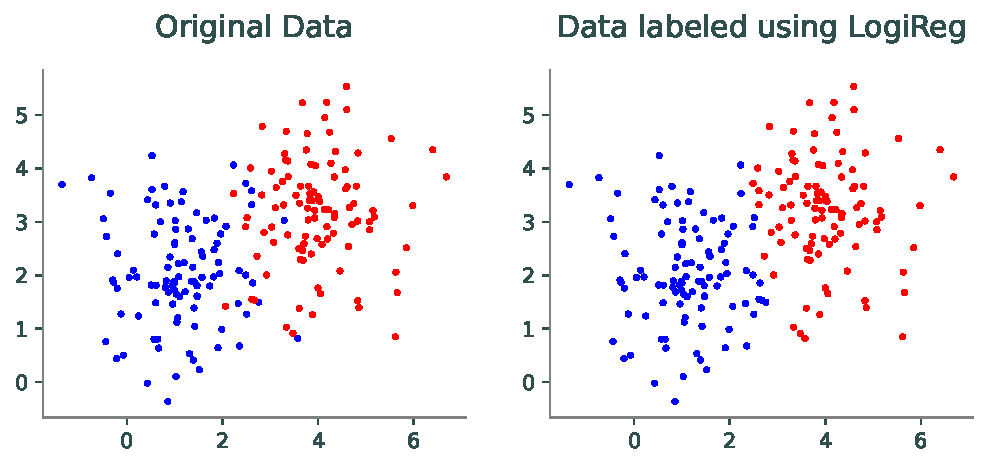
\includegraphics[width=.9\textwidth]{figures/prob3_test.pdf}
    \caption{In reality, these two distributions overlap a little, but the logistic regression model makes a clean divide between the two.}
    \label{fig:prob3}
\end{figure}


\section*{Statsmodels and Sklearn}

The module \li{statsmodels} contains a package that includes a logistic regression class called \li{Logit}.
A simple example of this class being implemented is as follows.
\begin{lstlisting}
>>> import statsmodels.api as sm

>>> model = sm.Logit(y, X).fit(disp=0)  # setting disp=0 turns off printed info
>>> probs = model.predict(X_test)  # list of probabilities, not labels
\end{lstlisting}
\li{Logit} does \emph{not} add a constant feature (column of $1$'s) to \li{X} by default, so in order to do so, you must apply the function \li{sm.add_constant()} to both \li{X} and \li{X\_test}.
In addition, the \li{.fit()} method does not regularize the problem by default, which may lead to some errors involving singular matrices.
To fix this, you can use the \li{.fit_regularized()} method instead of \li{.fit()}.

The module \li{sklearn} also has a package for logistic regression called \li{LogisticRegression}, which can be implemented as follows.

\begin{lstlisting}
>>> from sklearn.linear_model import LogisticRegression

>>> model = LogisticRegression(fit_intercept=True).fit(X, y)  # X before y
>>> labels = model.predict(X_test)  # predicted labels of X_test
\end{lstlisting}
\li{LogisticRegression} already regularizes the problem by default.
The parameter \li{fit_intercept} (which defaults to \li{False}) indicates whether you want to add a constant feature (column of $1$'s) to \li{X} and \li{X\_test}.

You can also use \li{sklearn} to score a logistic regression model.
After fitting an \li{sklearn} model, you can call \li{<model>.score(X_test, y_test)} to find the percentage of accuracy of the model's prediction for \li{X\_test}, given the true labels in \li{y\_test}.
Alternatively, you can use \li{sklearn.metrics.accuracy_score} to find the percentage of accuracy between a list of predicted labels and the list of true labels.
\begin{lstlisting}
>>> from sklearn.metrics import accuracy_score

>>> true_labels = [0, 1, 2, 3, 4]
>>> pred_labels = [0, 2, 2, 2, 4]  # predicted labels from logistic regression
>>> accuracy_score(true_labels, predicted_labels)
0.6
\end{lstlisting}

\section*{Support Vector Machines}

Support Vector Machines (SVM) are another type of classifier. It uses what is called the 'kernel trick' to handle nonlinear input spaces. It classifies data by finding an optimal hyperplane to split the data. 
\begin{lstlisting}
>>> from sklearn import svm

>>> svm = svm.SVC(kernel = 'linear').fit(X, y)
>>> labels = svm.predict(X_test)          # predicted labels of X_test
\end{lstlisting}


\begin{problem}
    The code to generate arrays \li{X}, \li{y}, \li{X\_test}, and \li{y\_test} is provided below.
    \li{X} and \li{X\_test} are each composed of $200$ draws from two $20$-dimensional multivariate normal distributions, one centered at $\boldsymbol{0}$, and the other centered at $\boldsymbol{2}$.
    
    Using each of \li{LogiReg}, \li{statsmodels}, \li{sklearn.LogisticRegression}, and \li{sklearn.svm}, train a logistic regression classifier on \li{X} and \li{y} to generate a list of predicted labels for \li{X\_test}.
    Then, using \li{y\_test}, print the accuracy scores for each trained model.
    Compare the accuracies and training/testing time for all four classifiers.
    Be sure to add a constant feature with each model.

    \begin{lstlisting}
    >>> # predefine the true beta
    >>> beta = np.random.normal(0, 7, 20)
        
    >>> # X is generated from 2 20-dim. multivariate normal dists.
    >>> X = np.concatenate(( 
            np.random.multivariate_normal(np.zeros(20), np.eye(20), 100), 
            np.random.multivariate_normal(np.ones(20)*2, np.eye(20), 100) 
            ))
    >>> np.random.shuffle(X)
    >>> # create y based on the true beta
    >>> pred = 1. / (1. + np.exp(-X @ beta))  
    >>> y = np.array( [1 if pred[i] >= 1/2 else 0 
                for i in range(pred.shape[0])] )
        
    >>> # X_test and y_test are generated similar to X and y
    >>> X_test = np.concatenate(( 
            np.random.multivariate_normal(np.zeros(20), np.eye(20), 100), 
            np.random.multivariate_normal(np.ones(20), np.eye(20), 100) 
            ))
    >>> np.random.shuffle(X_test)
    >>> pred = 1. / (1. + np.exp(-X_test @ beta))
    >>> y_test = np.array( [1 if pred[i] >= 1/2 else 0 
                for i in range(pred.shape[0])] )
    \end{lstlisting}
    Hint: Consider using the command \li{fit_regularized(disp = 0)} for the \li{statsmodels} case.
\end{problem}



\section*{Multiclass Logistic Regression}

Sometimes we may want to classify data into more than two categories, but so far we've only used logistic regression as a binary classifier.
The good news is that we can extend logistic regression to classify more than just two categories.

The more popular method for doing this is to generalize the logistic regression model to a multiclass setting.
This method is called \emph{multinomial logistic regression} or sometimes \emph{softmax regression}.
While standard logistic regression was based on the sigmoid function, multinomial logistic regression is based on the \emph{softmax function} $\softmax: \mathbb{R}^k \to (0,1)^k$, which is a multivariate version of the sigmoid function, given by

\begin{equation}
    \softmax(t_1,\dots,t_k) = \left(\frac{e^{t_1}}{\sum_{j=1}^k e^{t_j}}, \dots, \frac{e^{t_k}}{\sum_{j=1}^k e^{t_j}}\right).
\end{equation}

\noindent We will assume that $Y \mid X$ is categorically distributed as
\[
    \cat(p_1(X),\dots, p_k (X)) = \cat(\softmax(X\trans \bbeta_1, \dots, X\trans \bbeta_k))
\]
for some choice of vectors $\bbeta_1,\dots, \bbeta_k$, which we will estimate from the data.  Here
\[
p_i(X) = P(Y = i \mid X) = \frac{e^{X\trans \bbeta_i}}{\sum_{j=1}^k e^{X\trans \bbeta_j}} 
 = \frac{\logistic(X\trans \bbeta_i)}{\sum_{j=1}^k \logistic(X\trans \bbeta_j)}.
\]

Given a draw of length $n$ of the form $D = \{(\x_1,y_1),\dots, (\x_n,y_n)\}$, we wish to compute $\boldsymbol{\theta} = (\bbeta_1,\dots, \bbeta_k)$ where, without loss of generality, we may assume $\bbeta_k=\boldsymbol{0}$.
The maximum likelihood estimate of $\boldsymbol{\theta}$ is computed in a manner similar to the way it was for standard logistic regression.
A bit of math shows that

\begin{align*}
    \ell(\boldsymbol{\theta}\mid D) 
    & = - \sum_{i=1}^n \sum_{j = 1}^k \delta_{c_j} (y_i) \log (p_j(\x_i)) \\
    & = - \sum_{i=1}^n \sum_{j = 1}^k \delta_{c_j} (y_i) \log \left(  \frac{e^{\x_i\trans\bbeta_j}}{\sum_{m=1}^k e^{\x_i\trans\bbeta_m}} \right)
\end{align*}
where 
\[
    \delta_{c_j} (y_i) = \begin{cases}
    1 & \text{if $y_i = c_j$, the jth class}\\
    0 & \text{otherwise}. 
    \end{cases}
\]
This is a convex minimization problem with unique minimizer $\widehat{\boldsymbol{\theta}}$.
Once $\widehat{\boldsymbol{\theta}} = (\widehat{\bbeta_1},\dots, \widehat{\bbeta_k})$ is found, we have an estimate for the probability
\[
    P(Y=y \mid \x) \approx \frac{e^{\x\trans \widehat{\bbeta}_y}}{\sum_{j=1}^k e^{\x\trans \widehat{\bbeta}_j}}.
\]
From this, we can construct a classifier $\widehat{f}$ by setting $\widehat{f}(\x) = \text{argmax}_j P(Y=c_j \mid \x) $.  

Conveniently, \li{sklearn} has a very simple implementation of multinomial logistic regression that simply requires the argument \li{multi_class='multinomial'} when initiating a \li{LogisticRegression} model.
\begin{lstlisting}
    >>> from sklearn.linear_model import LogisticRegression

    >>> model = LogisticRegression(
                    multi_class='multinomial',
                    fit_intercept=True).fit(X, y) # add constant feature
\end{lstlisting}


\begin{problem}
    The Iris Dataset contains information taken from $150$ samples of $3$ different types of iris flowers (Setosa, Versicolor, and Virginica).
    The columns contain measurements for sepal length, sepal width, pedal length, and pedal width.
    Import the Iris Dataset and perform a train-test split on only the first two columns of the data with \li{test_size=0.4}.
    Train a multinomial logistic regression model using the training data with an added constant feature, and generate prediction labels for the test data.
    Plot the test data by color using your prediction labels. Also, print the model score.
    Reference code below for accessing the Iris Dataset and for using \li{train_test_split}.
\begin{lstlisting}
>>> import numpy as np
>>> from sklearn.model_selection import train_test_split

>>> iris = datasets.load_iris()

>>> X = iris.data[:, :2]  # we only take the first two features.
>>> y = iris.target

>>> X_train, X_test, y_train, y_test = train_test_split(X, y, test_size=0.4)
\end{lstlisting}
    Your plot should reflect Figure \ref{fig:iris}
\end{problem}

\begin{figure}[H]
    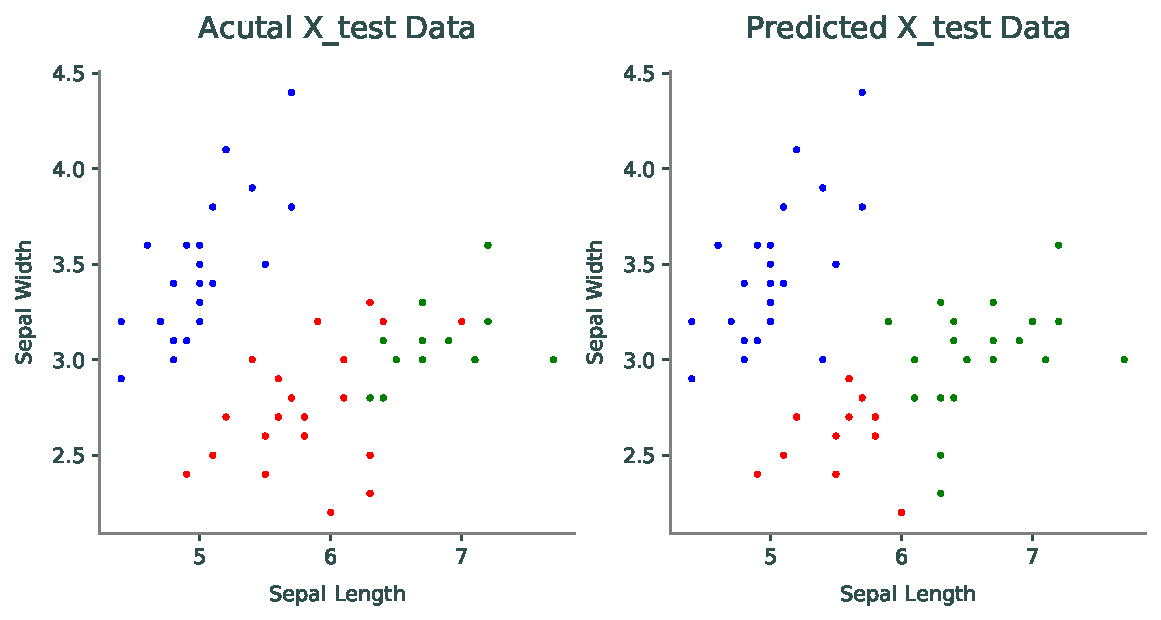
\includegraphics[width=.9\textwidth]{figures/plot_iris.pdf}
    \caption{Multinomial logistic regression attempt to categorize the Iris Dataset.}
    \label{fig:iris}
\end{figure}
